%%%%%%%%%%%%%%%%%%%%%%%%%%%%%%%%%%%%%%%%%%%%%%%%%%%%%%%%%%%%%%%%%%%%%%%%%%%%%%%
%
% SIINTEC Template Example Document
% Simpósio Internacional de Inovação e Tecnologia
% International Symposium on Innovative Technologies
%
% Author: Nelson Alves Ferreira Neto
% Email: nelsonafn@gmail.com
% Date: July 29, 2025
% Version: 1.0
%
% Description: Example document demonstrating the use of the SIINTEC LaTeX class
%              for symposium papers. This template illustrates the correct
%              formatting of academic articles according to the event guidelines.
%
% Features demonstrated:
%   - Title, author, and affiliation formatting with custom commands
%   - Abstract with keywords and abbreviations in single column
%   - Section hierarchy and automatic numbering
%   - Tables and figures with captions and cross-references
%   - Numbered mathematical equations
%   - Vancouver reference style with square brackets
%   - Two-column layout for main content
%   - Custom header with logo and ISSN
%
% Usage instructions:
%   1. Replace the example content with your article
%   2. Update title, authors, and affiliations using \siintectitle, \siintecauthor, \siintecaffil
%   3. Fill in the abstract, keywords, and abbreviations in \siintecabstract
%   4. Insert your sections, figures, tables, and references
%   5. Compile with pdflatex and bibtex (if using automatic references)
%
% Requirements:
%   - siintec.cls (event class)
%   - siintec.png (event logo)
%   - Images used in figures
%   - Reference file refs.bib
%
% 2025 Conference Theme:
%   "Quantum Technologies: The information revolution that will change the future"
%
%%%%%%%%%%%%%%%%%%%%%%%%%%%%%%%%%%%%%%%%%%%%%%%%%%%%%%%%%%%%%%%%%%%%%%%%%%%%%%%

% Loads the SIINTEC class (based on article, with custom formatting)
\documentclass{siintec}
% --- Ajustes para autores do authblk ---
\makeatletter
\renewcommand{\siintecauthor}[2][]{%
  \author[#1]{\siintecauthorfont #2}
}

\setlength{\affilsep}{0.35em}

\renewcommand\Authand{, }
\renewcommand\Authands{, }
\makeatother

%--------------------------- ARTICLE METADATA -------------------------------%

% Article title (max. 3 lines, Times 12pt bold, centered)
\siintectitle{SARA: Abordagem com LLMs para Revisão Sistemática da Literatura com Caso de Uso em Integração Clássico–Quântica para Comunicação Segura}

% Authors and affiliations (use [*] for corresponding author, [n] for multiple affiliations)
\siintecauthor[*,1]{Naiara Santos}
\siintecauthor[1,2]{Marcus Freire}
\siintecauthor[1]{Anderson Tomkelski}
\siintecauthor[1,2]{Thiago Mello}
\siintecauthor[2]{Maycon Peixoto}
\siintecauthor[1]{Ricardo Parizotto}
\siintecauthor[*,1]{João Souza}

\siintecaffil[1]{QuIIN – Quantum Industrial Innovation,Centro de Competência EMBRAPII CIMATEC em Tecnologias Quânticas,
SENAI CIMATEC, Salvador, Bahia, Brasil. }
\siintecaffil[2]{Instituto de Computação, Universidade Federal da Bahia (UFBA), Salvador, Bahia, Brasil}
%\siintecaffil[3]{Organization Name, Department Name, City, State, Country}
\siintecaffil[*]{Corresponding author: SENAI CIMATEC; naiara.bonfim@fbter.org.br; joao.marcelo@fieb.org.br}

% Remove the default LaTeX date
\siintecdate

%--------------------------- BEGIN DOCUMENT ---------------------------------%

\begin{document}

%--------------------------- FRONT MATTER -----------------------------------%

% Formatted abstract (single column, then two columns)
% Parameters: {abstract text}{keywords}{abbreviations}
\siintecabstract
{Este trabalho apresenta o SARA (Sistema de Análise e Revisão semi-Automatizada), uma abordagem que integra Large Language Models (LLMs), modelagem de tópicos e busca semântica para apoiar Revisões Sistemáticas da Literatura (RSL). Como caso de uso, aplicou-se o SARA ao domínio da integração entre redes clássicas e comunicações quânticas seguras, contemplando \textit{Quantum Key Distribution} (QKD) e \textit{Post-Quantum Cryptography} (PQC); realizando deduplicação, pré-seleção, categorização e ranqueamento de artigos, priorizando publicações com maior potencial de contribuição científica. Os resultados indicam predominância de estudos sobre QKD, seguidos por PQC e abordagens híbridas, com destaque para telecomunicações, IoT e sistemas críticos. A SARA demonstrou identificar publicações alinhadas às consultas do pesquisador e estudos conceitualmente próximos, evidenciando seu potencial para otimizar processos de RSL em áreas tecnológicas emergentes.}
{Revisão Sistemática da Literatura. Modelagem de Tópicos. Busca Semântica. LLMs. Comunicações Quânticas Seguras.}
{SARA, Sistema de Análise e Revisão semi-Automatizada. LLM, Large Language Model. QKD, Quantum Key Distribution. PQC, Post-Quantum Cryptography. RSL, Revisão Sistemática da Literatura. PLN, Processamento de Linguagem Natural.}


%--------------------------- MAIN CONTENT -----------------------------------%

% Main section (bold, 12pt, automatic numbering)
\section{Introdução}
% Main text: Times 12pt, 1.5 spacing, justified, two columns
O volume de publicações científicas tem crescido exponencialmente nas últimas décadas, impulsionado pela disseminação digital e pela ampla acessibilidade a bases de dados especializadas, tornando mais desafiadora a execução de Revisões Sistemáticas da Literatura (RSL), que demandam tempo, rigor metodológico e elevado esforço humano. Com o avanço dos Modelos de Linguagem de Grande Escala (Large Language Models – LLMs), como o GPT e suas variantes, cresce o número de estudos explorando seu uso para otimizar diferentes fases da RSL \cite{scherbakov2025emergence_RSL}, sendo que abordagens híbridas, combinando LLMs e revisão humana, demonstram reduzir o tempo de triagem e extração de dados, mantendo elevada precisão \cite{yehybrid_RSL}, enquanto técnicas baseadas em embeddings contextualizados e aprendizado profundo mostram eficácia na pré-classificação e agrupamento temático de artigos, acelerando as etapas iniciais de triagem \cite{alchokr2022supporting_RSL}.

Nos últimos anos, o volume de publicações relacionadas a tecnologias quânticas aplicadas à segurança da informação tem crescido de forma acelerada, acompanhando a maturação de protótipos e a realização de testes em cenários de campo como o exemplo da Rede Metropolitana Quântica do Rio \cite{temporao2024rio}. Esse avanço é impulsionado tanto pela corrida para viabilizar comunicações invioláveis quanto pela preocupação com o chamado “apocalipse quântico”, a possibilidade de que computadores quânticos suficientemente poderosos comprometam algoritmos criptográficos atualmente em uso \cite{abughanem2025ibm}. Entre as abordagens para mitigar esse risco destacam-se: (i) a \textit{Quantum Key Distribution} (QKD), que utiliza um canal quântico para compartilhar chaves criptográficas entre dois pares de forma segura, explorando princípios fundamentais da mecânica quântica e apoiando-se em um canal clássico para autenticação \cite{qi2021bennett}; e (ii) a \textit{Post-Quantum Cryptography} (PQC), que emprega algoritmos de cifragem baseados em problemas matemáticos considerados difíceis até mesmo para computadores quânticos \cite{alagic2022status}. Embora distintas na implementação, QKD e PQC perseguem o mesmo objetivo: garantir que a comunicação permaneça segura frente a adversários dotados de capacidades quânticas.

Nesse contexto, a necessidade de ferramentas que realizam pré-seleção, classificação e ranqueamento de publicações com base em critérios semânticos torna-se evidente. O presente trabalho propõe e aplica uma abordagem semi-automatizada para RSL, que denominamos o SARA (Sistema de Análise e Revisão semi-Automatizada), que permita a triagem inicial e categorização de artigos científicos relevantes, integrando técnicas de Processamento de Linguagem Natural (PLN) e LLMs, para esse caso de uso do SARA nosso foco é em três objetivos principais: (i) integração de sistemas clássicos com tecnologias quânticas, incluindo PQC, QKD ou ambas; (ii) modelagem dos principais tópicos recorrentes na área; e (iii) recuperação semântica dos artigos mais relevantes, priorizando aqueles com maior potencial de contribuição científica.

\section{Trabalhos Relacionados}

A pesquisa em métodos computacionais para apoiar RSL tem evoluído rapidamente, acompanhando o avanço de técnicas de PLN, aprendizado profundo e, mais recentemente, LLMs \cite{galli2025large}. As abordagens variam em escopo e grau de automação, abrangendo desde fluxos de trabalho baseados em machine learning tradicional até sistemas interativos com capacidade de compreensão semântica. Apesar de avanços expressivos, observa-se que poucos trabalhos integram de forma plena mecanismos de ranqueamento orientados por perguntas do pesquisador, modelagem de tópicos e busca semântica contextual, elementos fundamentais para priorizar publicações de maior relevância em domínios complexos.

\begin{table}[ht]
\centering
\caption{
Comparação de trabalhos relacionados.  
Colunas: (1) Uso de LLM; (2) Ranqueamento por perguntas; (3) Modelagem de tópicos; (4) Busca semântica; (5) Ano de publicação.
}
\label{tab:relatedwork}
\begin{tabular}{c c c c c c}
\hline
\textbf{Ref.} & \textbf{(5)} & \textbf{(1)} & \textbf{(2)} & \textbf{(3)} & \textbf{(4)} \\
\hline
\cite{pham2021text} & 2021 & Não & Não & Sim & Sim \\
\cite{tsang2022artificial} & 2022 & Não & Parcial & Sim & Sim \\
\cite{ramesh2022automated} & 2022 & Não & Parcial & Não & Parcial \\
\cite{yehybrid_RSL}& 2024 & Não & Não & Sim & Parcial \\
\cite{galli2025large} & 2025 & Sim & Sim & Sim & Sim \\
\textbf{SARA} & 2025 & \textbf{Sim} & \textbf{Sim} & \textbf{Sim} & \textbf{Sim} \\
\hline
\end{tabular}
\end{table}


Conforme mostrado na Tabela~\ref{tab:relatedwork}, \cite{pham2021text} apresentam um workflow semi-automatizado com Random Forest, SVD, LDA e embeddings, reduzindo a carga de triagem em 55--63\%.
\cite{tsang2022artificial} combinam embeddings BERT, BERTopic e recuperação semântica, permitindo consultas interativas para filtragem.
\cite{yehybrid_RSL} aplicam análise bibliométrica e \textit{topic modeling} para mapear tendências, porém sem recuperação semântica baseada em embeddings.
\cite{ramesh2022automated} revisam \textit{active learning} para triagem, com feedback humano influenciando a priorização.
Por fim, \cite{galli2025large} integram LLMs para sumarização, classificação e ranqueamento guiado por perguntas, aliando busca semântica e modelagem de tópicos.

Diante desse panorama, a abordagem SARA proposta neste trabalho diferencia-se por combinar, de forma integrada, os quatro elementos-chave observados na literatura: uso de LLMs, ranqueamento orientado por perguntas do pesquisador, modelagem de tópicos recorrentes e recuperação semântica avançada. Embora \cite{galli2025large} também explorem ranqueamento guiado por perguntas, sua aplicação ocorre de forma independente à modelagem de tópicos, limitando o potencial de ajuste contextual da pontuação dos artigos. No SARA, as respostas às perguntas do pesquisador são diretamente vinculadas à estrutura temática extraída do corpus, permitindo reponderação dinâmica dos pesos semânticos e priorização mais precisa dos estudos relevantes. Além disso, o fluxo de pré-seleção e categorização foi desenhado para otimizar a etapa inicial da RSL, reduzindo o esforço humano e aumentando a precisão na identificação de estudos pertinentes. A seguir, a Seção~\ref{sec:metodologia} descreve detalhadamente a arquitetura, as técnicas empregadas e o processo de implementação da SARA.



\section{Metodologia}
\label{sec:metodologia}
A metodologia adotada é concebida para realizar uma RSL de forma semiautomatizada, visando reduzir o esforço humano nas etapas iniciais de triagem e organização de artigos. O fluxo metodológico, ilustrado na Figura~\ref{fig:fluxo_sara}, compreende quatro macroetapas: (i) coleta e deduplicação dos dados; (ii) pré-seleção baseada em LLM; (iii) modelagem de tópicos; e (iv) busca semântica. Esse processo, denominado SARA, abrange desde a deduplicação inicial até a priorização final dos artigos, incorporando modelagem de tópicos e ranqueamento semântico guiado por perguntas do pesquisador.

\begin{figure}[ht]
    \centering

    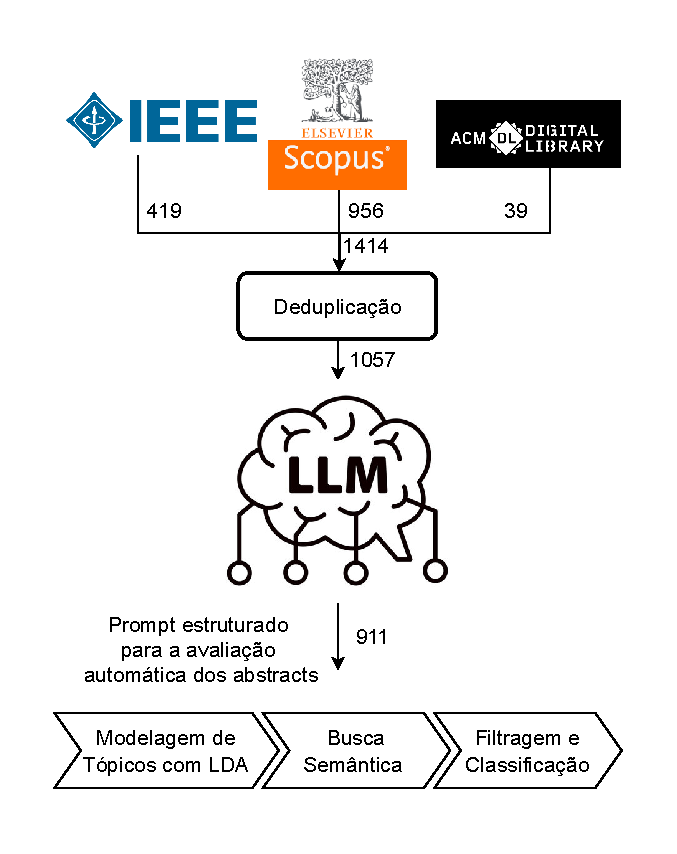
\includegraphics[width=0.95\linewidth]{img/fluxo_sara.pdf}

        \caption{Fluxo metodológico da abordagem SARA. O processo inicia-se com a deduplicação do corpus, seguido de avaliação automática dos \textit{abstracts} por meio de prompt estruturado, modelagem de tópicos com LDA e busca semântica. Na etapa final, realiza-se a filtragem, classificação e ranqueamento dos artigos com base nas respostas às perguntas do pesquisador.}

    \label{fig:fluxo_sara}
\end{figure}

\subsection{Construção da String de Busca}
Como etapa preliminar, foi elaborada uma string de busca padronizada para maximizar a relevância dos resultados nas três bases consultadas (IEEE Xplore, Scopus e ACM Digital Library), direcionando o retorno para publicações alinhadas à linha de pesquisa. A consulta foi construída com operadores booleanos aplicados ao campo abstract:

\textit{(("Quantum Key Distribution" OR "QKD" OR "Quantum Cryptography" OR "Quantum Key Exchange" OR "Post-Quantum Cryptography" OR "PQC" OR "Quantum-Resistant Cryptography" OR "Quantum-Safe Cryptography")  
AND  
("integration" OR "interoperability" OR "migration" OR "framework" OR "compatibility" OR "communication protocol"))
}

O primeiro conjunto de termos refere-se às tecnologias alvo desta revisão: QKD, PQC e variações terminológicas associadas à criptografia quântica e pós-quântica; enquanto o segundo conjunto abrange conceitos ligados à integração e interoperabilidade de sistemas, assegurando que os resultados contemplassem estudos focados tanto no aspecto tecnológico quanto na aplicação em arquiteturas de comunicação.

Os resultados obtidos nas três bases foram exportados em formato CSV, consolidados e submetidos a um processo de deduplicação com base na correspondência de título, ano e DOI (quando disponível, pois nem todos os artigos possuíam esse identificador), resultando em um total de 1.057 artigos.

\subsection{Pré-seleção automatizada com o LLM (GPT)}
Foi elaborado um prompt estruturado para a avaliação automática dos abstracts, abrangendo cinco critérios: (1) tecnologias mencionadas — PQC, QKD, ambas ou nenhuma; (2) integração com rede clássica — implementação real, simulação, proposta conceitual ou nenhuma integração; (3) aplicação ou protótipo — presença e descrição; (4) desafios técnicos — quantitativos, qualitativos ou ambos; e (5) domínios de aplicação — até dez áreas possíveis.

Cada critério recebeu uma pontuação específica, sendo as questões (1) e (2) são definidos como critérios eliminatórios — caso ambos sejam classificados como “Nenhuma”, o artigo recebe pontuação de –10 e é automaticamente excluído da RSL. As questões (3), (4) e (5), por sua vez, são de caráter classificatório: caso seja identificada no abstract alguma aplicação, desafio técnico ou domínio de aplicação explicitamente descrito, é atribuído 1 ponto para cada ocorrência. Ao final, os artigos são ranqueados com base no somatório das pontuações, resultando em um conjunto reduzido de 911 trabalhos com potencial relevância.

\subsection{Modelagem de tópicos (Latent Dirichlet Allocation – LDA)}
Para a etapa de organização temática, empregou-se o algoritmo Latent Dirichlet Allocation (LDA)\cite{blei2003latent_LDA}, visando à detecção automática de tópicos predominantes no conjunto de artigos pré-selecionados. Os abstracts são previamente processados em seguida submetidos à modelagem LDA, o que permite a identificação de tópicos latentes e o agrupamento dos estudos em macrotemas representativos da área \cite{egger2022topic_bertTOPIC}.

\subsection{Busca semântica baseada em embeddings}
Após a etapa de modelagem de tópicos com LDA, os resultados são utilizados para orientar a recuperação de documentos semanticamente relevantes. Para essa tarefa, adota-se o modelo pré-treinado all-MiniLM-L6-v2, disponibilizado pela biblioteca Sentence-Transformers, responsável por converter tanto os abstracts quanto as consultas do pesquisador em representações vetoriais densas. A similaridade entre documentos e consultas é calculada por meio da métrica de cosseno, permitindo identificar publicações relacionadas mesmo na ausência de coincidência lexical exata \cite{seo2022ta_sentece_BERT, kamil2025advances_semantic_search}.

A fim de potencializar a qualidade da recuperação, cada representação textual foi enriquecida com informações complementares extraídas automaticamente por um LLM (ChatGPT-4), de modo a incluir aspectos essenciais sobre a aplicação, o tipo de tecnologia abordada (PQC, QKD ou ambas) e o nível de integração proposto (real, simulação ou conceitual). Esse enriquecimento semântico aumentou a capacidade do modelo em capturar nuances contextuais, resultando em recomendações mais precisas e alinhadas aos objetivos da revisão.

O fluxo completo da abordagem SARA, desde a deduplicação inicial até a priorização final dos artigos, é apresentado na Figura~\ref{fig:fluxo_sara}, destacando as etapas de modelagem de tópicos e ranqueamento semântico guiado por perguntas do pesquisador, modelagem de tópicos e a busca semântica. Na próxima seção, apresentam-se os resultados obtidos com a aplicação desse fluxo, discutindo-se tanto o desempenho das etapas individuais quanto as contribuições do sistema como um todo para a execução de Revisões Sistemáticas da Literatura no domínio de integração entre QKD e PQC.

\section{Resultados e Discussões}
A aplicação da abordagem SARA resultou na identificação e categorização de um conjunto significativo de artigos distribuídos entre as tecnologias consideradas nesta revisão: QKD, PQC e abordagens híbridas que combinam ambas e como pré-requisito fosse integrado na rede clássica, ou seja, nossa infraestrutura e tecnologias usadas atualmente. 

Como apresentado na Figura~\ref{fig:qtd_artigos_tecnologia}, observou-se predominância de publicações relacionadas exclusivamente à QKD (497 artigos), seguida por PQC (306 artigos) e, em menor número, estudos que abordam simultaneamente QKD e PQC (71 artigos). Essa distribuição evidencia não apenas o estágio mais avançado da literatura sobre QKD, mas também a crescente, embora ainda limitada, exploração de soluções híbridas que integram as duas tecnologias, aspecto particularmente relevante para esta pesquisa, dado o foco em estratégias de integração segura entre sistemas clássicos e quânticos.

\begin{figure}[t!]
    \centering
    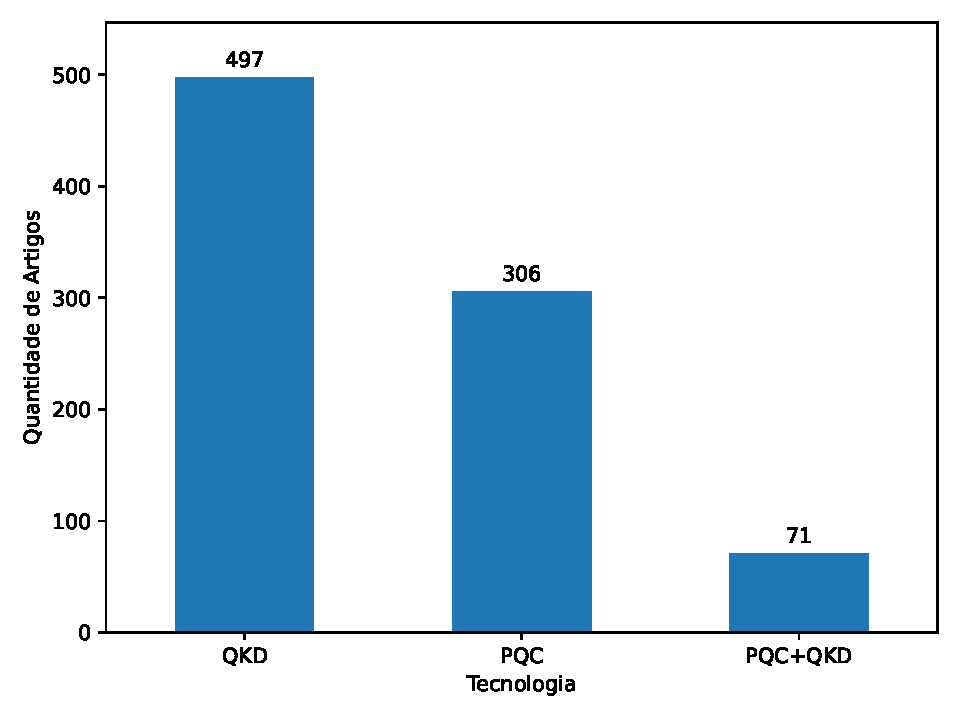
\includegraphics[width=0.95\linewidth]{img/q1.pdf}
    \caption{Distribuição dos artigos identificados por tecnologia: QKD, PQC e abordagens híbridas (QKD+PQC).}
    \label{fig:qtd_artigos_tecnologia}
\end{figure}

A análise dos domínios de aplicação (Figura~\ref{fig:dominios_aplicacao}) mostra predominância do setor de telecomunicações e 5G, refletindo a relevância de QKD e PQC para proteger canais de alta capacidade e baixa latência. Em seguida, destacam-se IoT/Edge, governo/defesa, data centers/cloud e sistemas via satélite, evidenciando o interesse em reforçar a segurança de redes críticas e infraestruturas sensíveis. Áreas como blockchain/DLT, sistemas industriais, setor financeiro e veículos conectados também indicam um amplo potencial de adoção dessas tecnologias no ecossistema digital.

\begin{figure}[t!]
    \centering
    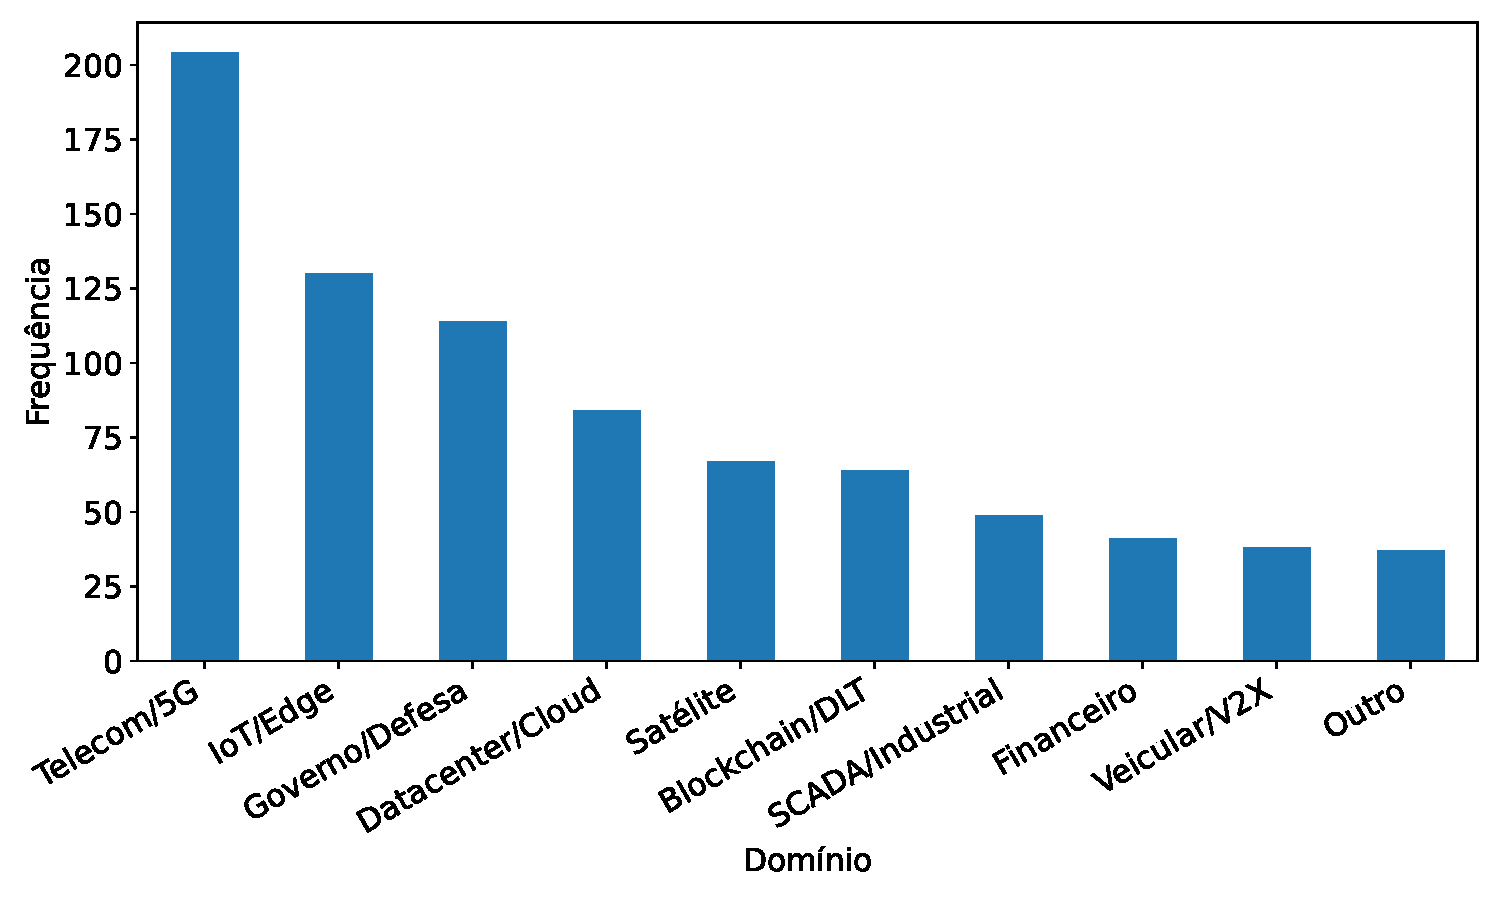
\includegraphics[width=1\linewidth]{img/q5_dominios.pdf}
    \caption{Distribuição dos artigos por domínio de aplicação das tecnologias QKD e PQC.}
    \label{fig:dominios_aplicacao}
\end{figure}

Para avaliar a capacidade da abordagem SARA em identificar publicações alinhadas a consultas específicas do pesquisador, foi formulada a pergunta: \textit{“What research applies quantum key distribution (QKD) or post-quantum cryptography (PQC) in 5G or telecommunications networks?”}. A busca semântica, utilizando embeddings vetoriais e cálculo de similaridade por cosseno, retornou um conjunto de artigos ranqueados de acordo com sua proximidade semântica em relação à consulta. A Figura~\ref{fig:busca_semantica} apresenta a projeção bidimensional (PCA) desse espaço vetorial, onde os pontos em azul representam os artigos selecionados como mais relevantes e o ponto marcado em vermelho indica a posição vetorial da pergunta no mesmo espaço. Os pontos em cinza correspondem a artigos não selecionados. Esse resultado demonstra que a SARA não apenas localiza publicações que compartilham termos com a consulta, mas também aquelas que apresentam relação conceitual, mesmo com vocabulário distinto, atribuindo um grau quantitativo de similaridade que permite priorizar as leituras mais pertinentes.

\begin{figure}[ht]
    \centering
    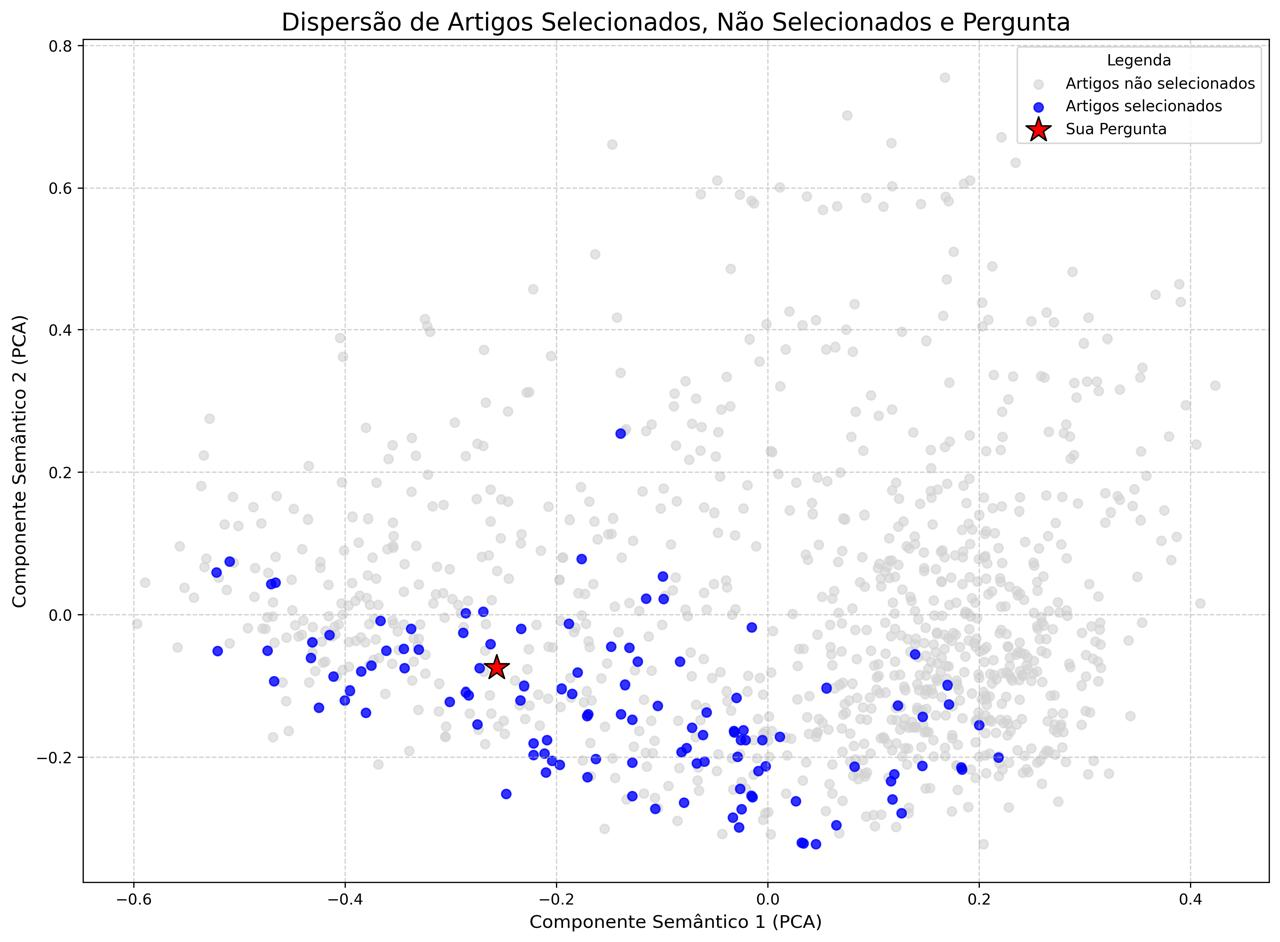
\includegraphics[width=1\linewidth]{img/busca_semantica.jpeg}
    \caption{Projeção bidimensional (PCA) do espaço vetorial resultante da busca semântica  para a consulta “What research applies quantum key distribution (QKD) or post-quantum cryptography (PQC) in 5G or telecommunications networks?”. Pontos azuis representam artigos selecionados como mais relevantes, pontos cinza indicam artigos não selecionados e a estrela vermelha corresponde à posição da consulta no espaço semântico.}
    \label{fig:busca_semantica}
\end{figure}

Em síntese, os resultados confirmam que a SARA integra de forma eficaz modelagem de tópicos, enriquecimento semântico e ranqueamento por perguntas, otimizando a seleção e priorização de artigos em RSL. O sistema demonstrou capacidade de recuperar publicações alinhadas às consultas e identificar estudos conceitualmente relacionados, mesmo sem correspondência lexical. A predominância de telecomunicações e 5G reforça a relevância de QKD e PQC para a segurança de redes críticas, enquanto as soluções híbridas despontam como campo promissor. Esses achados consolidam a SARA como ferramenta útil para pesquisas em áreas tecnológicas emergentes.

\section{Conclusão}

Este trabalho apresentou a abordagem SARA, um fluxo metodológico semi-automatizado para apoio a RSL, integrando modelagem de tópicos, enriquecimento semântico e ranqueamento orientado por perguntas, com foco no domínio da integração entre redes clássicas e comunicações quânticas seguras (QKD e PQC). A aplicação da SARA demonstrou que a combinação de técnicas de NLP e LLMs pode reduzir significativamente o esforço humano na triagem e priorização de artigos, mantendo alta relevância nos resultados. As análises evidenciaram que, além de recuperar publicações diretamente alinhadas às consultas do pesquisador, o sistema é capaz de identificar estudos conceitualmente relacionados, mesmo na ausência de termos coincidentes, aspecto essencial em áreas com terminologia técnica diversificada e em rápida evolução.

Entre as contribuições principais, destacam-se: (i) a integração de modelagem de tópicos e busca semântica para organização e filtragem do corpus; (ii) o uso de enriquecimento textual via LLMs para aumentar a densidade semântica e melhorar a recuperação; e (iii) a capacidade de ranqueamento dinâmico baseado em perguntas, permitindo ao pesquisador direcionar o foco da revisão. O estudo também reforçou a relevância das tecnologias QKD e PQC para setores críticos, com ênfase em telecomunicações, IoT e sistemas híbridos.

Como trabalhos futuros, propõe-se: (i) ampliar a base de dados analisada, incorporando múltiplas fontes indexadas e literatura cinzenta; (ii) explorar outras arquiteturas de embeddings e modelos de retrieval-augmented generation (RAG) para melhorar a precisão da busca semântica; (iii) incorporar métricas quantitativas de avaliação, como precision, recall e F1-score, para mensurar objetivamente o desempenho; e (iv) adaptar a SARA a outros domínios científicos, validando sua generalização e comparando-a com abordagens tradicionais de RSL.


%--------------------------- ACKNOWLEDGEMENTS -------------------------------%

%\section*{Agradecimentos}
%Este trabalho foi parcialmente financiado pelo projeto QuIIN Integração CV-QKD com Redes Clássicas apoiado pelo QuIIN - Inovação Industrial Quântica, Centro de Competência EMBRAPII CIMATEC em Tecnologias Quânticas, com recursos financeiros do PPI IoT/Manufatura 4.0 do edital MCTI número 053/2023, firmado com a EMBRAPII. Este estudo também contou com financiamento, em parte, pela Coordenação de Aperfeiçoamento de Pessoal de Nível Superior - Brasil (CAPES) - Código de Financiamento 001, e pelo Conselho Nacional de Desenvolvimento Científico e Tecnológico (CNPq), Brasil, sob a concessão nº 403231/2023-0.

%--------------------------- BIBLIOGRAPHY -----------------------------------%

% Only keep the bibliography command, style is now set by the class
\section*{References}
\bibliography{refs}

\end{document}
